% Weekly meeting report — Beamer deck
% Compile with: tectonic weekly_meeting.tex
\documentclass[aspectratio=169]{beamer}
\usetheme{metropolis}
\metroset{block=fill, progressbar=frametitle, numbering=fraction, sectionpage=none}
\definecolor{mCharcoal}{HTML}{2B2D33}
\definecolor{mCoral}{HTML}{E4572E}
\definecolor{mTeal}{HTML}{1B998B}
\setbeamercolor{frametitle}{bg=mCharcoal, fg=white}
\setbeamercolor{progress bar}{fg=mCoral}
\setbeamercolor{title separator}{fg=mCoral}
\setbeamercolor{alerted text}{fg=mCoral}
\setbeamercolor{example text}{fg=mTeal}
\setbeamercolor{block title alerted}{fg=white, bg=mCoral}
\setbeamercolor{normal text}{fg=mCharcoal, bg=white}
\setbeamertemplate{caption}{\raggedright\insertcaption\par}

\usepackage{tikz}
\usetikzlibrary{positioning, arrows.meta, shapes.geometric, calc, backgrounds, fit}
\usepackage{booktabs}
\usepackage{graphicx}
\graphicspath{{figures/}}

% palette
\definecolor{silo}{RGB}{68,114,196}
\definecolor{chain}{RGB}{112,173,71}
\definecolor{cost}{RGB}{196,78,82}
\definecolor{coord}{RGB}{38,70,120}

\title[Cost of Patient Autonomy in Federated Learning]{The Cost of Patient Autonomy in\\Federated Learning for Healthcare}
\subtitle{Weekly meeting report}
\author{Thuan Nhan}
\institute{Ph.D.\ Program in Data Science}
\date{July 10, 2026}

\begin{document}

\begin{frame}[plain]\titlepage\end{frame}

% ------------------------------------------------------------------
\begin{frame}{The one-sentence version}
\begin{block}{What I am doing}
Hospitals want to build medical AI \emph{together} without ever sharing patient
records. Patients should be able to \emph{opt out at any time}. \\[4pt]
\textbf{My work measures what that ``opt out at any time'' actually costs} ---
in model accuracy, and in system overhead.
\end{block}
\vfill
\begin{itemize}
\item Everyone has \emph{built} systems that let patients control their data.
\item \textbf{Nobody has measured the price} of giving them that control.
\item That measurement is the thesis.
\end{itemize}
\end{frame}

% ------------------------------------------------------------------
\begin{frame}{The problem, in plain terms}
\begin{columns}[T]
\begin{column}{0.55\textwidth}
\begin{itemize}
\item Good medical AI needs data from \textbf{many hospitals}.
\item But privacy law forbids \textbf{pooling patient records} in one place.
\item \textbf{Federated learning} is the workaround:
\begin{itemize}
  \item each hospital trains on its \emph{own} data,
  \item only the \emph{model} is shared --- never the data.
\end{itemize}
\end{itemize}
\end{column}
\begin{column}{0.42\textwidth}
\begin{block}{Analogy}
Students each do their homework at home and share only \emph{what they learned}.
A coordinator averages the lessons. No one's homework ever leaves the house.
\end{block}
\end{column}
\end{columns}
\vfill
\footnotesize\textit{Add a blockchain on top so each \textbf{patient} can grant or revoke
consent in real time --- and now the training population keeps changing.}
\end{frame}

% ------------------------------------------------------------------
\begin{frame}{The big picture: the whole set-up}
\centering
\resizebox{0.97\textwidth}{!}{%
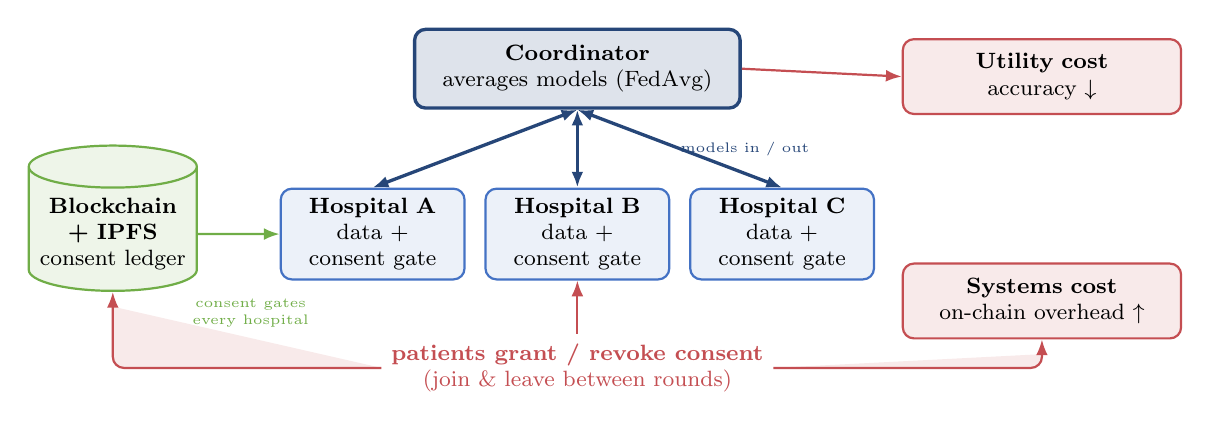
\begin{tikzpicture}[font=\footnotesize,
  silo/.style={rounded corners, draw=silo, thick, fill=silo!10, align=center, text width=2.1cm, minimum height=1.05cm},
  coord/.style={rounded corners, draw=coord, very thick, fill=coord!15, align=center, text width=3.9cm, minimum height=1cm},
  ledger/.style={cylinder, shape border rotate=90, aspect=0.25, draw=chain, thick, fill=chain!12, align=center, text width=1.9cm, minimum height=1.4cm},
  cost/.style={rounded corners, draw=cost, thick, fill=cost!12, align=center, text width=3.3cm, minimum height=0.95cm},
  ex/.style={{Latex[length=2mm]}-{Latex[length=2mm]}, thick, coord},
  ar/.style={-{Latex[length=2mm]}, thick}]

\node[coord] at (0,2.6) (co) {\textbf{Coordinator}\\ averages models (FedAvg)};
\node[silo] at (-2.6,0.5) (h1) {\textbf{Hospital A}\\ data + consent gate};
\node[silo] at (0,0.5) (h2) {\textbf{Hospital B}\\ data + consent gate};
\node[silo] at (2.6,0.5) (h3) {\textbf{Hospital C}\\ data + consent gate};
\node[ledger] at (-5.9,0.5) (led) {\textbf{Blockchain + IPFS} consent ledger};
\node[align=center, text=cost] at (0,-1.2) (churn) {\textbf{patients grant / revoke consent}\\ (join \& leave between rounds)};
\node[cost] at (5.9,2.5) (uc) {\textbf{Utility cost}\\ accuracy $\downarrow$};
\node[cost] at (5.9,-0.35) (sc) {\textbf{Systems cost}\\ on-chain overhead $\uparrow$};

% model exchange (data never leaves)
\draw[ex] (h1.north) -- (co.south);
\draw[ex] (h2.north) -- node[right, font=\tiny, text=coord]{~models in / out} (co.south);
\draw[ex] (h3.north) -- (co.south);

% consent layer controls the hospitals
\draw[ar, chain] (led.east) -- (h1.west);
\node[font=\tiny, text=chain, align=center] at (-4.15,-0.5) {consent gates\\ every hospital};

% churn feeds the data and the ledger
\draw[ar, cost] (churn.north) -- (h2.south);
\draw[ar, cost] (churn.west) -| (led.south);

% the two measured costs
\draw[ar, cost] (co.east) -- (uc.west);
\draw[ar, cost] (churn.east) -| (sc.south);
\end{tikzpicture}}

\vfill
{\footnotesize One knob --- the consent \textbf{churn} rate --- drives \emph{both}
costs at once. The thesis maps the trade-off between them.}
\end{frame}

% ------------------------------------------------------------------
\begin{frame}{What changed this week (a course-correction)}
\begin{columns}[T]
\begin{column}{0.48\textwidth}
\textbf{Before}
\begin{itemize}
\item Cervical-cancer dataset (858 rows).
\item Plus \emph{Synthea} synthetic patients for scale.
\end{itemize}
\vspace{4pt}
\textcolor{cost}{\textbf{Problems:}}
\begin{itemize}
\item Cervical data too small --- only \textbf{54} positive cases; a churn study needs more.
\item Synthetic data is too ``fake'' to measure real accuracy.
\end{itemize}
\end{column}
\begin{column}{0.48\textwidth}
\textbf{Now}
\begin{itemize}
\item One big \emph{real} hospital dataset:\\ \textbf{100{,}000 patients} (diabetes readmission).
\end{itemize}
\vspace{4pt}
\textcolor{chain}{\textbf{Why it is better:}}
\begin{itemize}
\item Big \emph{and} real --- does the job of both old sources.
\item Synthea kept only to \textbf{stress-test system scale}, where accuracy does not matter.
\end{itemize}
\end{column}
\end{columns}
\vfill
\footnotesize\textit{Same method, cleaner data. The approach did not change --- the measuring stick did.}
\end{frame}

% ------------------------------------------------------------------
\begin{frame}{Why this dataset is hard (and realistic)}
\begin{columns}[T]
\begin{column}{0.5\textwidth}
\textbf{1. A \emph{lot} of missing data}
\begin{itemize}\small
\item \texttt{weight}: \textbf{97\%} missing
\item glucose / A1C lab tests: \textbf{83--95\%} missing
\item medical specialty: \textbf{49\%} missing
\item payer code: \textbf{40\%} missing
\end{itemize}
\vspace{3pt}
{\footnotesize A missing test often means ``not ordered'' --- itself a clue, so we
keep it as its own category instead of dropping the patient.}
\end{column}
\begin{column}{0.5\textwidth}
\textbf{2. \emph{Highly} skewed labels}
\begin{itemize}\small
\item Only \textbf{11\%} of patients are readmitted within 30 days.
\item Predicting ``nobody gets readmitted'' scores \textbf{89\% accuracy} --- and is useless.
\end{itemize}
\vspace{3pt}
{\footnotesize So we \emph{never} judge by accuracy. We use \textbf{AUROC} and
\textbf{PR-AUC}, which stay honest under heavy imbalance.}
\end{column}
\end{columns}
\vfill
\centering{\footnotesize\textit{Messy + imbalanced = realistic clinical data --- a fair, hard stress test for the consent study.}}
\end{frame}

% ------------------------------------------------------------------
\begin{frame}{Result 1 --- our model is at ``state of the art''}
\begin{columns}[c]
\begin{column}{0.62\textwidth}
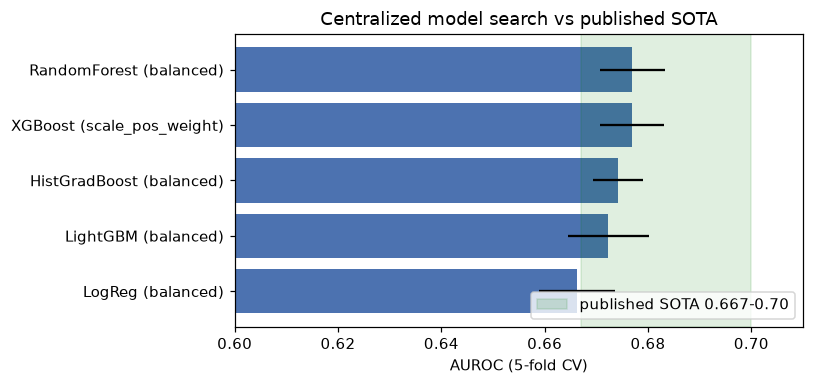
\includegraphics[width=\linewidth]{base_0}
\end{column}
\begin{column}{0.36\textwidth}
{\footnotesize \textbf{AUROC} = how well it ranks risk\\ (0.5 = coin flip, 1.0 = perfect).}
\vspace{6pt}
\begin{itemize}\small
\item RF / XGBoost: \textbf{0.677}
\item Logistic regression: 0.666
\item Best published: \textbf{0.667--0.70}
\end{itemize}
\vspace{4pt}
{\footnotesize We \textbf{match the best published results} --- the task is simply hard.}
\end{column}
\end{columns}
\vfill
{\scriptsize Sources: Strack \textit{et al.}~2014 (dataset); 2025 EHR study --- XGBoost 0.667
(PubMed~40385730); Liu \textit{et al.}, \textit{J.~Medical AI}. Links on ``Sources'' slide.}
\end{frame}

% ------------------------------------------------------------------
\begin{frame}{Result 2 --- federated learning works}
\begin{itemize}\small
\item Across \textbf{3 hospitals}, federation recovers \textbf{almost all} the accuracy of pooling data.
\item \textbf{5 averaging recipes} are \textbf{basically tied} --- but \textcolor{mCoral}{\textbf{SCAFFOLD breaks}} (drops to 0.625) when hospitals differ a lot.
\end{itemize}
\vspace{2pt}
\centering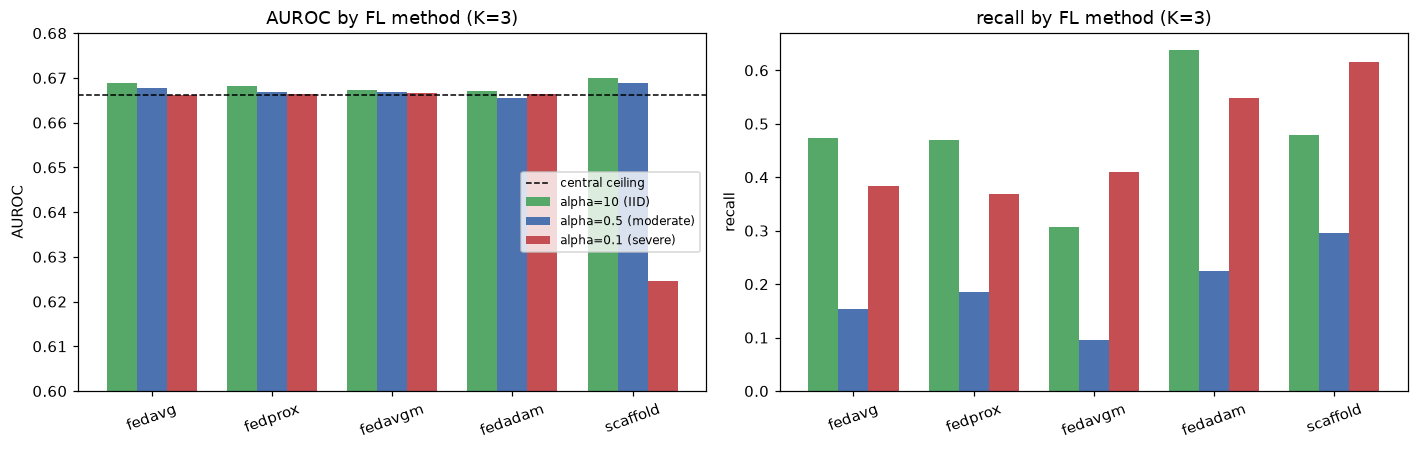
\includegraphics[width=0.97\linewidth]{base_1}
\end{frame}

% ------------------------------------------------------------------
\begin{frame}{Result 3 --- the key finding: consent ``churn''}
\begin{columns}[c]
\begin{column}{0.55\textwidth}
{\footnotesize Accuracy drop when patients withdraw consent:}
\begin{center}\small
\begin{tabular}{lc}
\toprule
Way patients leave & drop \\
\midrule
Leave temporarily, then return & \textcolor{mTeal}{$-0.003$} \\
Leave for good, at random & \textcolor{mTeal}{$-0.007$} \\
The ``sick'' patients leave first & \textcolor{mCoral}{$-0.021$} \\
A whole hospital leaves & \textcolor{mCoral}{\textbf{$-0.059$}} \\
\bottomrule
\end{tabular}
\end{center}
\end{column}
\begin{column}{0.43\textwidth}
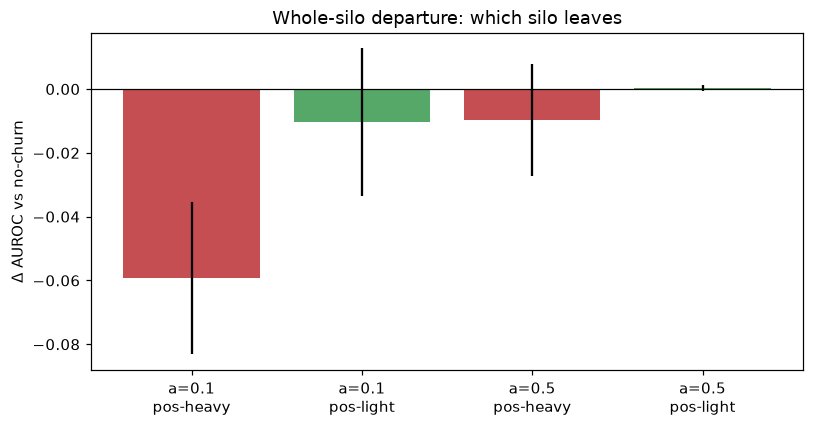
\includegraphics[width=\linewidth]{churn_1}
\end{column}
\end{columns}
\vspace{2pt}
\begin{alertblock}{The punchline}
\textbf{WHO leaves matters far more than HOW MANY leave} --- losing a whole hospital hurts
\textbf{8$\times$} more than the same number of random patients.
\end{alertblock}
\end{frame}

% ------------------------------------------------------------------
\begin{frame}{Result 3, in pictures --- per-patient churn}
\centering
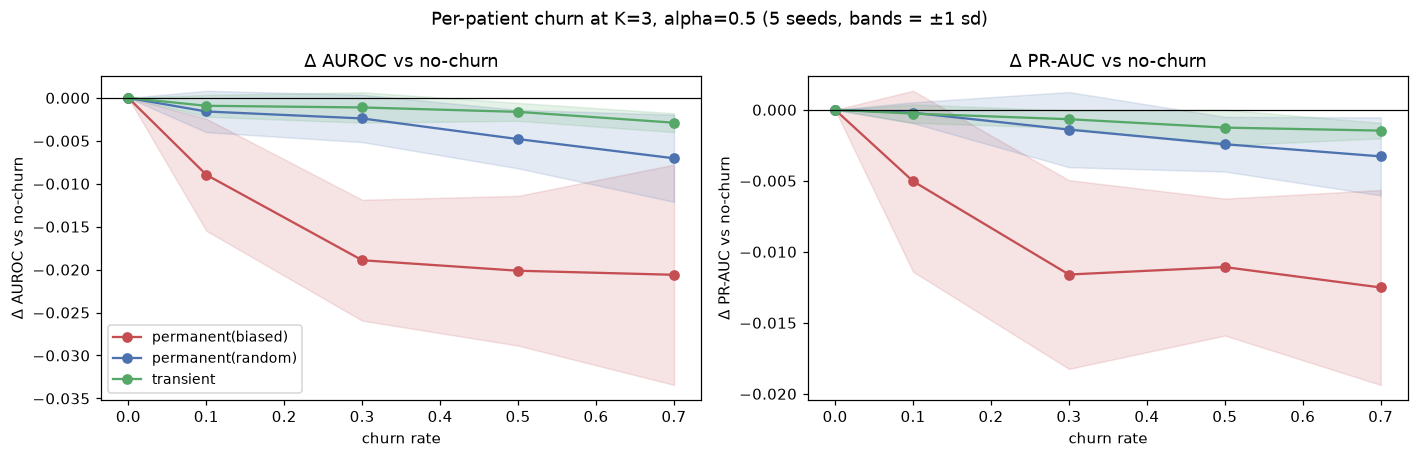
\includegraphics[width=0.97\linewidth]{churn_0}
\vfill
{\footnotesize \textcolor{mTeal}{\textbf{Green}} (leave \& return) and \textbf{blue} (random)
barely dip; \textcolor{mCoral}{\textbf{red}} (the ``sick'' leave first) falls \textbf{3$\times$}
further --- again, the cost is \emph{who} leaves, not how many.}
\end{frame}

% ------------------------------------------------------------------
\begin{frame}{Where Synthea fits now}
\begin{itemize}
\item The two costs share \textbf{one driver}: the rate at which patients change consent.
\item Every consent change = one \textbf{blockchain transaction} = system overhead.
\item \textbf{Synthea} lets us blow the patient population up to \textbf{real-hospital scale}
to measure that overhead (time, compute, bandwidth).
\item Here we \emph{ignore accuracy on purpose} --- we only care about system load.
\end{itemize}
\vfill
\begin{block}{Why this is clean}
Accuracy is measured on \emph{real} data (diabetes); system cost is measured at \emph{scale}
(Synthea); both are driven by the \emph{same} consent-churn knob.
\end{block}
\end{frame}

% ------------------------------------------------------------------
\begin{frame}{How the two datasets are used (no overlap of jobs)}
\centering
\resizebox{0.97\textwidth}{!}{%
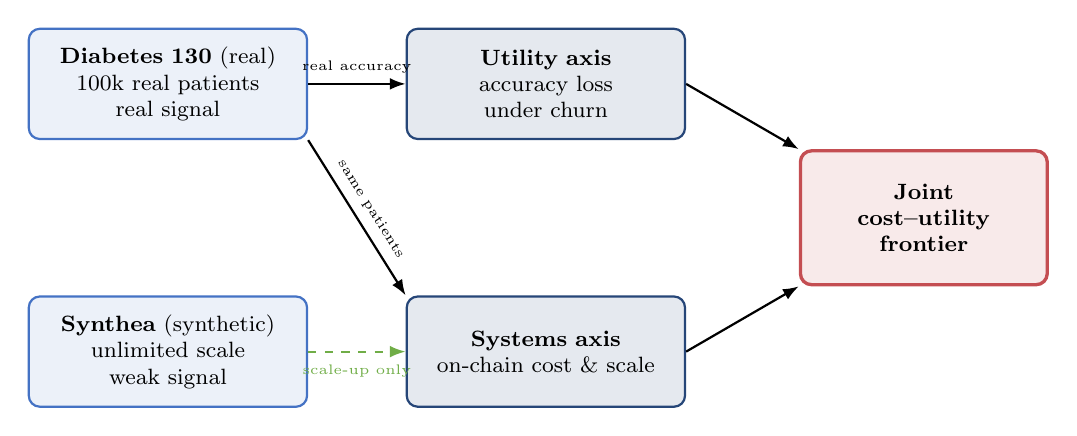
\begin{tikzpicture}[font=\footnotesize,
  src/.style={rounded corners, draw=silo, thick, fill=silo!10, align=center, text width=3.3cm, minimum height=1.4cm},
  axis/.style={rounded corners, draw=coord, thick, fill=coord!12, align=center, text width=3.3cm, minimum height=1.4cm},
  fr/.style={rounded corners, draw=cost, very thick, fill=cost!12, align=center, text width=2.9cm, minimum height=1.7cm},
  ar/.style={-{Latex[length=2mm]}, thick}]

\node[src] at (0,1.7) (dia) {\textbf{Diabetes 130} (real)\\ 100k real patients\\ real signal};
\node[src] at (0,-1.7) (syn) {\textbf{Synthea} (synthetic)\\ unlimited scale\\ weak signal};

\node[axis] at (4.8,1.7) (ua) {\textbf{Utility axis}\\ accuracy loss under churn};
\node[axis] at (4.8,-1.7) (sa) {\textbf{Systems axis}\\ on-chain cost \& scale};

\node[fr] at (9.6,0) (fr) {\textbf{Joint}\\ \textbf{cost--utility}\\ \textbf{frontier}};

\draw[ar] (dia.east) -- node[above,font=\tiny]{real accuracy} (ua.west);
\draw[ar] (dia.south east) -- node[sloped,above,font=\tiny]{same patients} (sa.north west);
\draw[ar, dashed, chain] (syn.east) -- node[below=1pt,font=\tiny, text=chain]{scale-up only} (sa.west);
\draw[ar] (ua.east) -- (fr.north west);
\draw[ar] (sa.east) -- (fr.south west);
\end{tikzpicture}}
\vfill
{\footnotesize \textbf{Diabetes} carries the real-accuracy curve \emph{and} the same-population
cost curve (the joint frontier); \textbf{Synthea} only pushes the systems axis to hospital
scale, where accuracy does not matter. The same churn knob drives both axes.}
\end{frame}

% ------------------------------------------------------------------
\begin{frame}{What is actually new here}
\begin{itemize}
\item The blockchain + federated system is the \textbf{instrument} --- already built and published.
\item The contribution is the \textbf{map}:
\end{itemize}
\begin{center}
\emph{As patients exercise autonomy, how much accuracy do we lose, and how much
system overhead do we pay?}
\end{center}
\begin{itemize}
\item[$\Rightarrow$] the \textbf{cost--utility frontier} of patient autonomy, and
\item[$\Rightarrow$] the finding that \textbf{who leaves} $>$ \textbf{how many leave}, and
\item[$\Rightarrow$] the point where per-patient on-chain consent \textbf{stops scaling}.
\end{itemize}
\vfill
\footnotesize\textit{Not ``we built a system'' (done before) --- but ``we measured what it costs.''}
\end{frame}

% ------------------------------------------------------------------
\begin{frame}{Next steps}
\begin{enumerate}
\item \textbf{Bigger model} --- test whether a more powerful model makes the consent effects larger.
\item \textbf{System-cost axis} --- wire in the on-chain measurement (gas, latency, bandwidth per round).
\item \textbf{Combine both} --- one cost-vs-benefit map (the central result).
\item \textbf{Scale test} --- use Synthea to find where per-patient on-chain consent becomes impractical.
\end{enumerate}
\end{frame}

% ------------------------------------------------------------------
\begin{frame}{Sources}
\footnotesize
\textbf{Dataset}
\begin{itemize}
\item Strack \textit{et al.} (2014), ``Impact of HbA1c Measurement on Hospital Readmission
Rates: Analysis of 70{,}000 Clinical Database Patient Records,'' \textit{BioMed Research
International} --- the UCI ``Diabetes 130-US hospitals'' dataset.
\end{itemize}
\textbf{State-of-the-art 30-day readmission AUROC (0.667--0.70)}
\begin{itemize}
\item ``Predicting 30-Day Hospital Readmission in Patients with Diabetes Using ML on EHR
Data'' (2025) --- XGBoost AUROC 0.667.\\ \url{https://pubmed.ncbi.nlm.nih.gov/40385730/}
\item Liu \textit{et al.}, ``Comparison of ML models for predicting 30-day readmission rates
for patients with diabetes,'' \textit{Journal of Medical Artificial Intelligence}.\\
\url{https://jmai.amegroups.org/article/view/9179/html}
\item A 2024 six-model comparison reports CatBoost $\approx 0.70$ (upper end of the band).
\end{itemize}
\textbf{Our result:} best model (RandomForest / XGBoost) AUROC \textbf{0.677} --- inside the
published band, i.e.\ at state of the art.
\end{frame}

% ------------------------------------------------------------------
\begin{frame}{Takeaways}
\begin{enumerate}
\item Switched to a \textbf{big real dataset}; our model is \textbf{at state of the art} (0.68).
\item Federated learning \textbf{works} and is robust at our scale --- simplest method is fine.
\item Key finding: consent ``churn'' is \textbf{cheap} unless it \textbf{shifts who is in the
data} --- \textbf{who leaves $>$ how many leave}.
\end{enumerate}
\vfill
\begin{center}\large Thank you --- questions welcome.\end{center}
\end{frame}

\end{document}
